\documentclass[12pt, twoside]{article}
\usepackage[letterpaper, margin=1in, headsep=0.5in]{geometry}
\usepackage[english]{babel}
\usepackage[utf8]{inputenc}
\usepackage{amsmath}
\usepackage{amsfonts}
\usepackage{amssymb}
\usepackage{tikz}
%\usetikzlibrary{quotes, angles}

\usepackage{graphicx}
\usepackage{enumitem}
\usepackage{multicol}

\usepackage{fancyhdr}
\pagestyle{fancy}
\fancyhf{}
\renewcommand{\headrulewidth}{0pt} % disable the underline of the header

\usepackage{setspace}
%\linespread{1.75}

%\fancyhead[RE]{\thepage}
\fancyhead[R]{\thepage \\ Name: \hspace{3cm}}
\fancyhead[L]{BECA / Dr. Huson / 12.1 IB Math SL\\* 1 March 2019}

\begin{document}
\subsubsection*{Unit 5 Exam Part 1: Integral Calculus - with calculator}
 \begin{enumerate}

\subsubsection*{You may use a calculator on these problems \hfill [34 marks]}

\setstretch{1.5}

\item Let $f(x)=x^2$ and $g(x)=\sin(x+1)$.
  \begin{enumerate}
    \item Solve for $f(x)=g(x)$. \hfill [3]
    \item Find the area of the region enclosed by the graphs of $f$ and $g$.  \hfill [3]
  \end{enumerate}

\vspace{2cm}

\item Let $f(x)=6-x^2$. Part of the graph of $f$ is shown in the following diagram.
    \begin{center}
      \begin{tikzpicture}[xscale=1,yscale=0.8]
        \draw [thick, ->] (-3,0) -- (3,0) node [below] {$x$};
        \draw [thick, ->] (0,-2) -- (0,6) node [left] {$y$};
        \draw[thick, domain=-2.5:2.5] plot[samples=100](\x, {5-(\x)^2});
        \fill (-5^0.5, 0) circle[radius=0.05] node[above left]{$A$};
        \fill (5^0.5, 0) circle[radius=0.05] node[above right]{$B$};
      \end{tikzpicture}
    \end{center}
  \begin{enumerate}
    \item The graph crosses the $x$-axis at the points $A$ and $B$.\\
    Find the $x$-coordinate of $A$ and of $B$. \hfill [3]
    \item The region enclosed by the graph of $f$ and the $x$-axis is rotated $360^\circ$ about the $x$-axis. Find the volume of the solid formed.  \hfill [3]
  \end{enumerate}

\newpage

\item Let $f(x)=3\ln(x-2)$, for $x>2$. The following diagram shows part of the graph of $f$.
    \begin{center}
      \begin{tikzpicture}[xscale=0.6,yscale=1]
        \draw [thick, ->] (0,0) -- (11,0) node [below] {$x$};
        \draw [thick, ->] (0,-3) -- (0,3) node [left] {$y$};
        \draw[thick, domain=2.1:10] plot[samples=100](\x, {ln(\x-2)});
        \draw[thick] (8, -.15)node[below]{$8$} --(8,0.15);
      \end{tikzpicture}
    \end{center}
  \begin{enumerate}
    \item Find the equation of the vertical asymptote to the graph of $f$. \hfill [2]
    \item Find the $x$-intercept of the graph of $f$. \hfill [2]
    \item The region enclosed by the graph of $f$, the $x$-axis, and the line $x=8$ is rotated $360^\circ$ about the $x$-axis. Find the volume of the solid formed.  \hfill [3]
  \end{enumerate}

\newpage

\item Let $f(x)=-x^4+2x^3-\frac{1}{2}$, for $0 \leq x \leq 2$.

  \begin{enumerate}
    \item Sketch the graph of $f$. \hfill [3]
      \begin{center}
      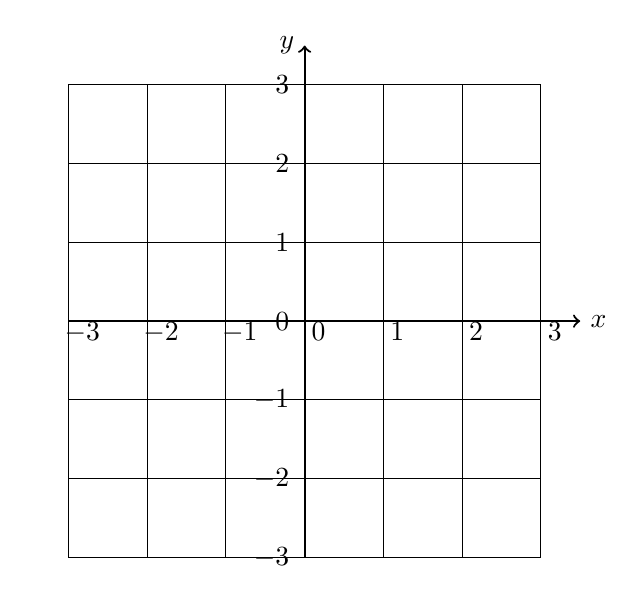
\begin{tikzpicture}%[scale=0.7]
        \draw [black, xstep=1.0cm, ystep=1.0cm] (-3,-3) grid (3,3);
        %\draw [gray, very thin, xstep=0.2cm, ystep=0.2cm] (0,-5) grid (10,5);
        \foreach \x in {-3,...,3}
        \draw[shift={(\x,0)},color=black] (0pt,-1pt) -- (0pt,3pt) node[below]  {$\quad \x$};
        \foreach \y in {-3,...,3}
        \draw[shift={(0,\y)},color=black] (2pt,0pt) -- (-2pt,0pt) node[left]  {$\y$};
        \draw [thick, ->] (-3,0) -- (3.5,0) node [right] {$x$};
        \draw [thick, ->] (0,-3) -- (0,3.5) node [left] {$y$};
        %\draw [thick,domain=0:2] plot(\x,{-(\x)^4+2*(\x)^3-0.5});
      \end{tikzpicture}
      \end{center}
    \item Solve for $f(x)=0$. \hfill [2]
    \item The region enclosed by the graph of $f$ and the $x$-axis is rotated $360^\circ$ about the $x$-axis. Find the volume of the solid formed.  \hfill [3]
  \end{enumerate}

\newpage

\item The graph of $y=(x-1)\sin x$, for $0 \leq x \leq \frac{5 \pi}{2}$, is shown below.
      \begin{center}
        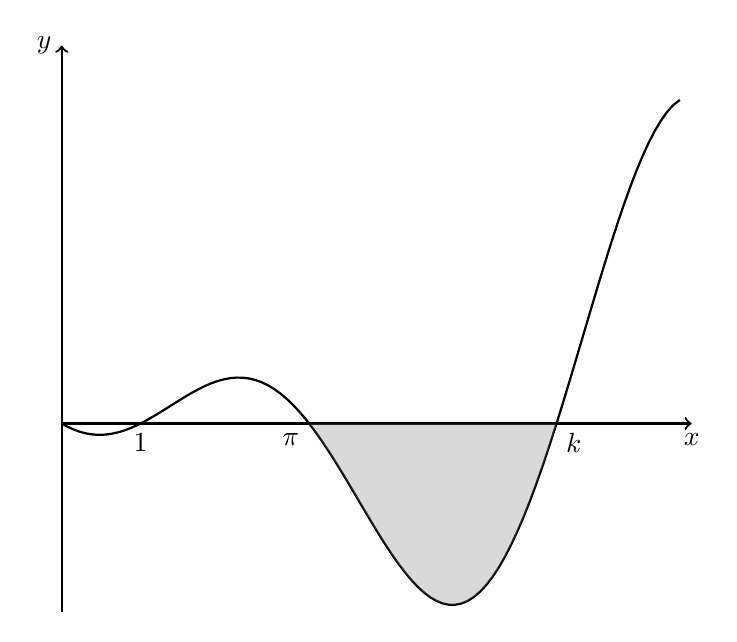
\begin{tikzpicture}[xscale=1,yscale=0.6]
          \draw [thick, ->] (0,0) -- (8,0) node [below] {$x$};
          \draw [thick, ->] (0,-4) -- (0,8) node [left] {$y$};
          \draw[thick, domain=0:7.85] plot[samples=100](\x, {(\x-1)*sin(\x r)});
          \draw (1, 0)node[below]{$1$};
          \draw (3.14, 0)node[below left]{$\pi$};
          \draw (6.28, 0)node[below right]{$k$};
          \fill[gray,opacity=.3] plot[domain=3.1416:6.283](\x, {(\x-1)*sin(\x r)});
          %\draw (1.5,1) node {$\mathbf{R}$};
        \end{tikzpicture}
      \end{center}
      \begin{enumerate}
        \item The graph has $x$-intercepts at $0,1, \pi, \text{ and }k$.
          Find $k$. \hfill [2]
        \item The shaded region is rotated $360^\circ$ about the $x$-axis. Let $V$ be the volume of the solid formed.\\
        Write down an expression for $V$. \hfill [3]
        \item Find $V$.  \hfill [2]
  \end{enumerate}

\newpage
\subsubsection*{Unit 5 Exam Part 2: Integral Calculus - without calculator}
\subsubsection*{No Calculator section \hfill [38 marks]}

\item Let $f(x)=x^2$.
  \begin{enumerate}
    \item Find $\int_1^2 (f(x))^2 \,\mathrm{d}x$ \hfill [4]
    \item The following diagram shows part of the graph of $f$.
      \begin{center}
        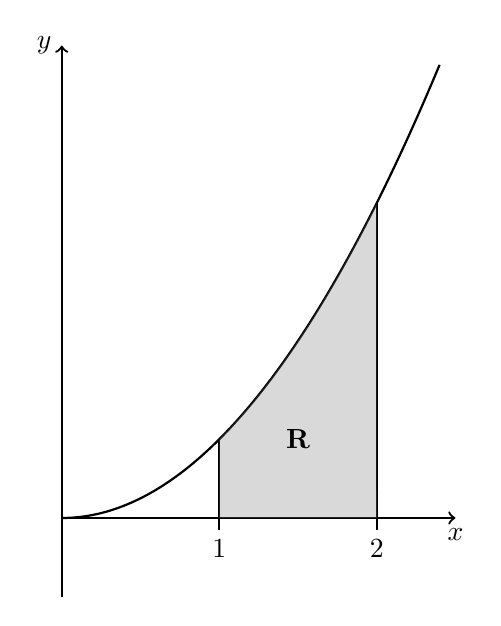
\begin{tikzpicture}[xscale=2,yscale=1]
          \draw [thick, ->] (0,0) -- (2.5,0) node [below] {$x$};
          \draw [thick, ->] (0,-1) -- (0,6) node [left] {$y$};
          \draw[thick, domain=0:2.4] plot[samples=100](\x, {(\x)^2});
          \draw[thick] (1, -.15)node[below]{$1$} --(1,1);
          \draw[thick] (2, -.15)node[below]{$2$} --(2,4);
          \fill[gray,opacity=.3] (1,0)--plot[domain=1:2](\x, {\x*\x})--(2,0);
          \draw (1.5,1) node {$\mathbf{R}$};
        \end{tikzpicture}
      \end{center}
    The shaded region $R$ is enclosed by the graph of $f$, the $x$-axis, and the lines $x=1$ and $x=2$.\\
    Find the volume of the solid formed when $R$ is revolved $360^\circ$ about the $x$-axis.  \hfill [2]
  \end{enumerate}

\end{enumerate}
\end{document}
